This is the interface to the GMII subsystem, and runs almost entirely
on the RX_CLK clock. The FIFO herein is only for conversion between
the potentially-different clock domains present external (RX_CLK) and
internal to the FPGA. There is no overflow-detection logic because the
output of the FIFO is free-running, that is it is always outputting
data as rapidly as it is put-in.

\begin{figure}
\label{gmii}
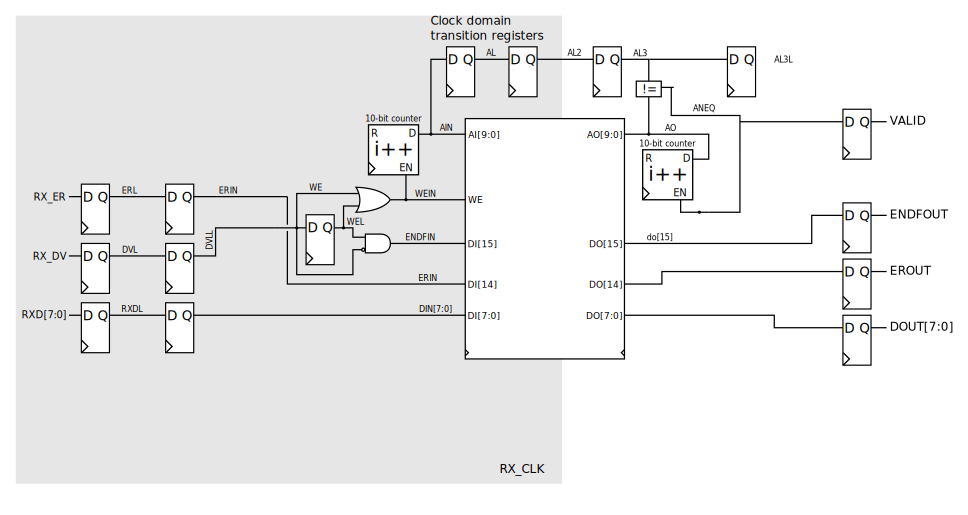
\includegraphics[scale=0.7]{gmii.svg}
\caption{Interface for GMII/PHY}
\end{figure}

We register the input RXD, RX_DV and RX_ER signals and then place them
into a fifo. The FIFO is actually 16-bits wide, with the lower [7:0]
being the registerd DV and the top bits being
\begin{itemize}
\item  D[15] : ENDF -- end frame signal. 
\item  D[14] : ER   -- error during the RX of this frame (from the PHY)
\end{itemize}

The input system writes into its FIFO. To signal the end of a frame,
it writes one extra word following the data, where D[15] (ENDF) =
1. Should this last word have it's ERF bit set, the
corresponding errors occurded during the RX of this frame and thus it
should be discarded.

Note that when \signal{AIN} = \signal{AO} then the fifo is empty;
similary, AIN is incremented following each write, so AIN = 1 when the
fifo is storing 1 word (at AIN=0).

The WEIN signal is ORed after a register, such that it stays high for
an extra tick following the end of a data write segment. ENDFIN is
structured to only be toggled on this last write.

AL and AL2 provide clock-synchronization between the RXCLK and CLK
clock domains. 

The output side is relatively simple, with \signal{VALID} asserting
whether or not the bytes present on the \signal{ENDFOUT},
\signal{EROUT}, and \signal{DOUT} bytes are valid.
